% !TeX program = xelatex
\documentclass[UTF8,11pt,a4paper,fontset=none]{ctexart}
\usepackage[margin=23mm,headheight=16pt,footskip=13mm]{geometry}
\usepackage{fontspec}
\setmainfont{Noto Sans}
\setsansfont{Noto Sans}
\setmonofont[Scale=0.85]{DejaVu Sans Mono}
\setCJKmainfont{Noto Sans CJK TC}
\setCJKsansfont{Noto Sans CJK TC}
\setCJKmonofont{Noto Sans Mono CJK TC}
\usepackage{amsmath,graphicx,booktabs,tabularx,longtable,array,multirow}
\usepackage[table]{xcolor}
\usepackage{enumitem,fancyhdr,tcolorbox,caption,float,pdflscape}
\usepackage{hyperref,xurl}
\definecolor{navy}{HTML}{16324F}
\definecolor{teal}{HTML}{087F8C}
\definecolor{light}{HTML}{EFF5F8}
\definecolor{muted}{HTML}{536578}
\definecolor{amber}{HTML}{8F5310}
\hypersetup{unicode=true,colorlinks=true,linkcolor=navy,urlcolor=teal,citecolor=teal,
  pdftitle={Saccade v1：追蹤流程與這一輪的結果},
  pdfauthor={Saccade v1 專案},pdfsubject={目的、實際畫面、跨資料集結果與速度取捨}}
\urlstyle{same}
\renewcommand{\contentsname}{目錄}
\renewcommand{\refname}{證據與參考文件}
\ctexset{section={format=\Large\bfseries\sffamily\color{navy}},
  subsection={format=\large\bfseries\sffamily\color{navy}},
  subsubsection={format=\normalsize\bfseries\sffamily}}
\clubpenalty=10000
\widowpenalty=10000
\setlength{\parindent}{2em}
\setlength{\parskip}{0.35em}
\linespread{1.18}
\setlength{\emergencystretch}{1.5em}
\setlength{\tabcolsep}{5pt}
\renewcommand{\arraystretch}{1.30}
\newcolumntype{Y}{>{\raggedright\arraybackslash}X}
\newcolumntype{P}[1]{>{\raggedright\arraybackslash}p{#1}}
\setlist[itemize]{leftmargin=1.7em,itemsep=0.25em,topsep=0.35em}
\setlist[enumerate]{leftmargin=1.9em,itemsep=0.3em,topsep=0.35em}
\captionsetup{font=small,labelfont={bf,color=navy},skip=8pt}
\pagestyle{fancy}\fancyhf{}
\fancyhead[L]{\small\sffamily\color{muted}Saccade v1｜目的・實作・結果}
\fancyhead[R]{\small\sffamily\color{muted}圖解版 v1.5}
\fancyfoot[L]{\scriptsize\color{muted}2026-11-12｜程式基準 3cbaa518f0dc}
\fancyfoot[R]{\small\thepage}
\renewcommand{\headrulewidth}{0.4pt}
\newtcolorbox{finding}[1][]{colback=light,colframe=teal,boxrule=0.7pt,
  arc=1mm,left=3mm,right=3mm,top=2mm,bottom=2mm,#1}
\newcommand{\code}[1]{\texttt{\detokenize{#1}}}
\newcommand{\status}[1]{\textbf{#1}}
\newcommand{\source}[1]{\par\noindent{\footnotesize\color{muted}來源：#1}\par}
\newcommand{\reportbase}{3cbaa518f0dc37d691404e95ed85c0109c81130d}
\begin{document}
\noindent{\small\sffamily\color{teal}SACCADE v1・第一輪專案筆記}\par
\vspace{4mm}
\noindent{\LARGE\bfseries\sffamily\color{navy}從畫面找人，\par 到持續追蹤同一個人}\par
\vspace{3mm}
\noindent{\large\color{muted}這一輪為什麼做、做出了什麼，以及結果怎麼看。}\par
\vspace{5mm}

\section{把「找到人」接成「持續追蹤」}
一張畫面裡把人框出來，只回答了「人在哪裡」。影片追蹤還要回答：\textbf{下一張畫面中的這個人，是否仍是剛才那個人？} 人會移動、互相遮住，攝影機也可能晃動；這些變化都會讓身份接續變難。

Saccade v1 把這些工作接成一條能跑完的流程。CPU 讀入畫面、安排工作、取回結果；中間影像、模型特徵和追蹤狀態留在 GPU。這樣設計是為了減少中間資料往返，讓找人、估計運動和接續身份能持續工作。

\begin{figure}[H]
\centering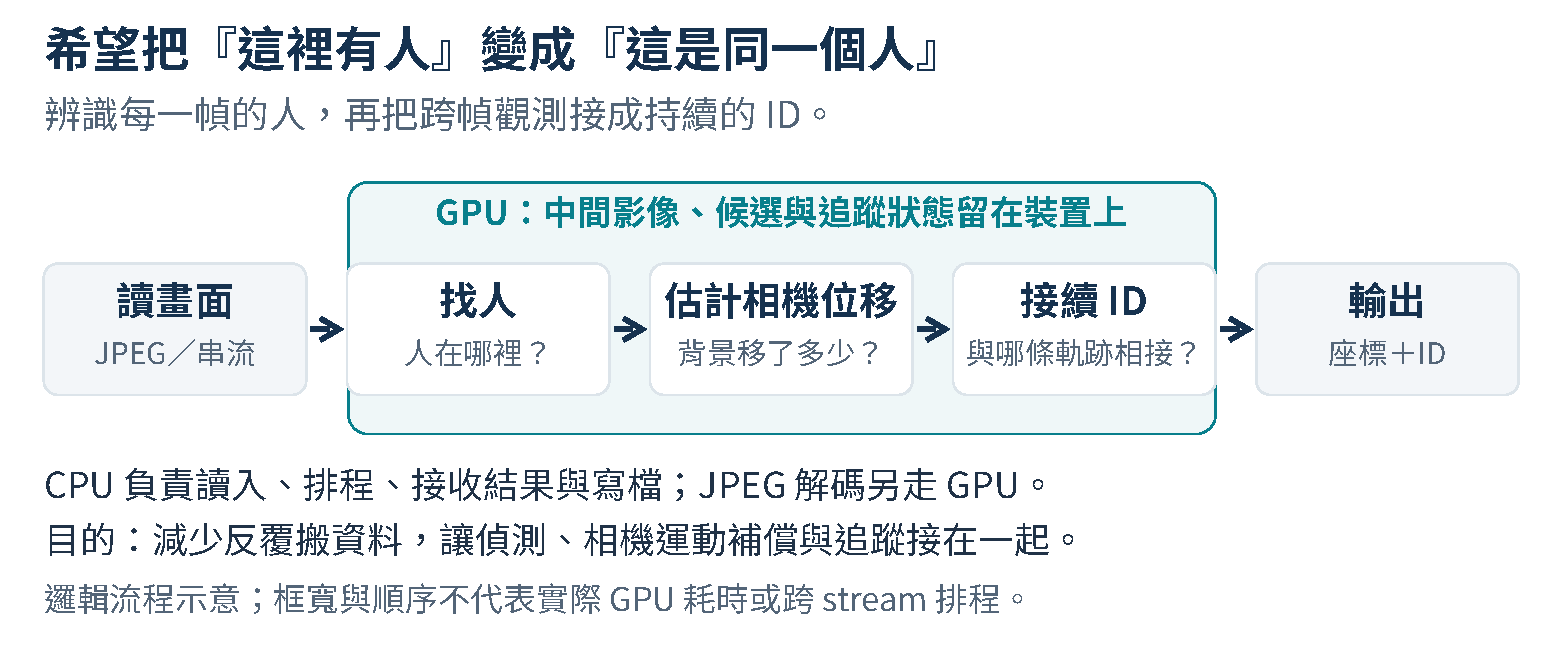
\includegraphics[width=\textwidth]{assets/story-pipeline.pdf}
\caption{先看每一步要解決什麼。方框是工作順序示意，寬度不代表時間。}
\end{figure}

\begin{finding}
\textbf{這輪主要回答三個問題：}\par
流程能不能完整接通？換模型後，哪些資料追得比較好？為了這些差異，多花了多少計算時間？
\end{finding}

後面先看實際畫面，再看品質與速度圖。完整設定、數字與驗證細節放在後段和保留的技術版；這裡先說清楚每個結果的意思。\cite{tracking,reference}

\clearpage
\section{畫面上的框和 ID，要怎麼看}
下圖取自已經產生的 MOT17-10 展示影片。框表示系統當下追蹤的目標，ID 是用來接續身份的編號。三張畫面中的 \textbf{ID 71}，都是既有輸出的真實記錄。

\begin{figure}[H]
\centering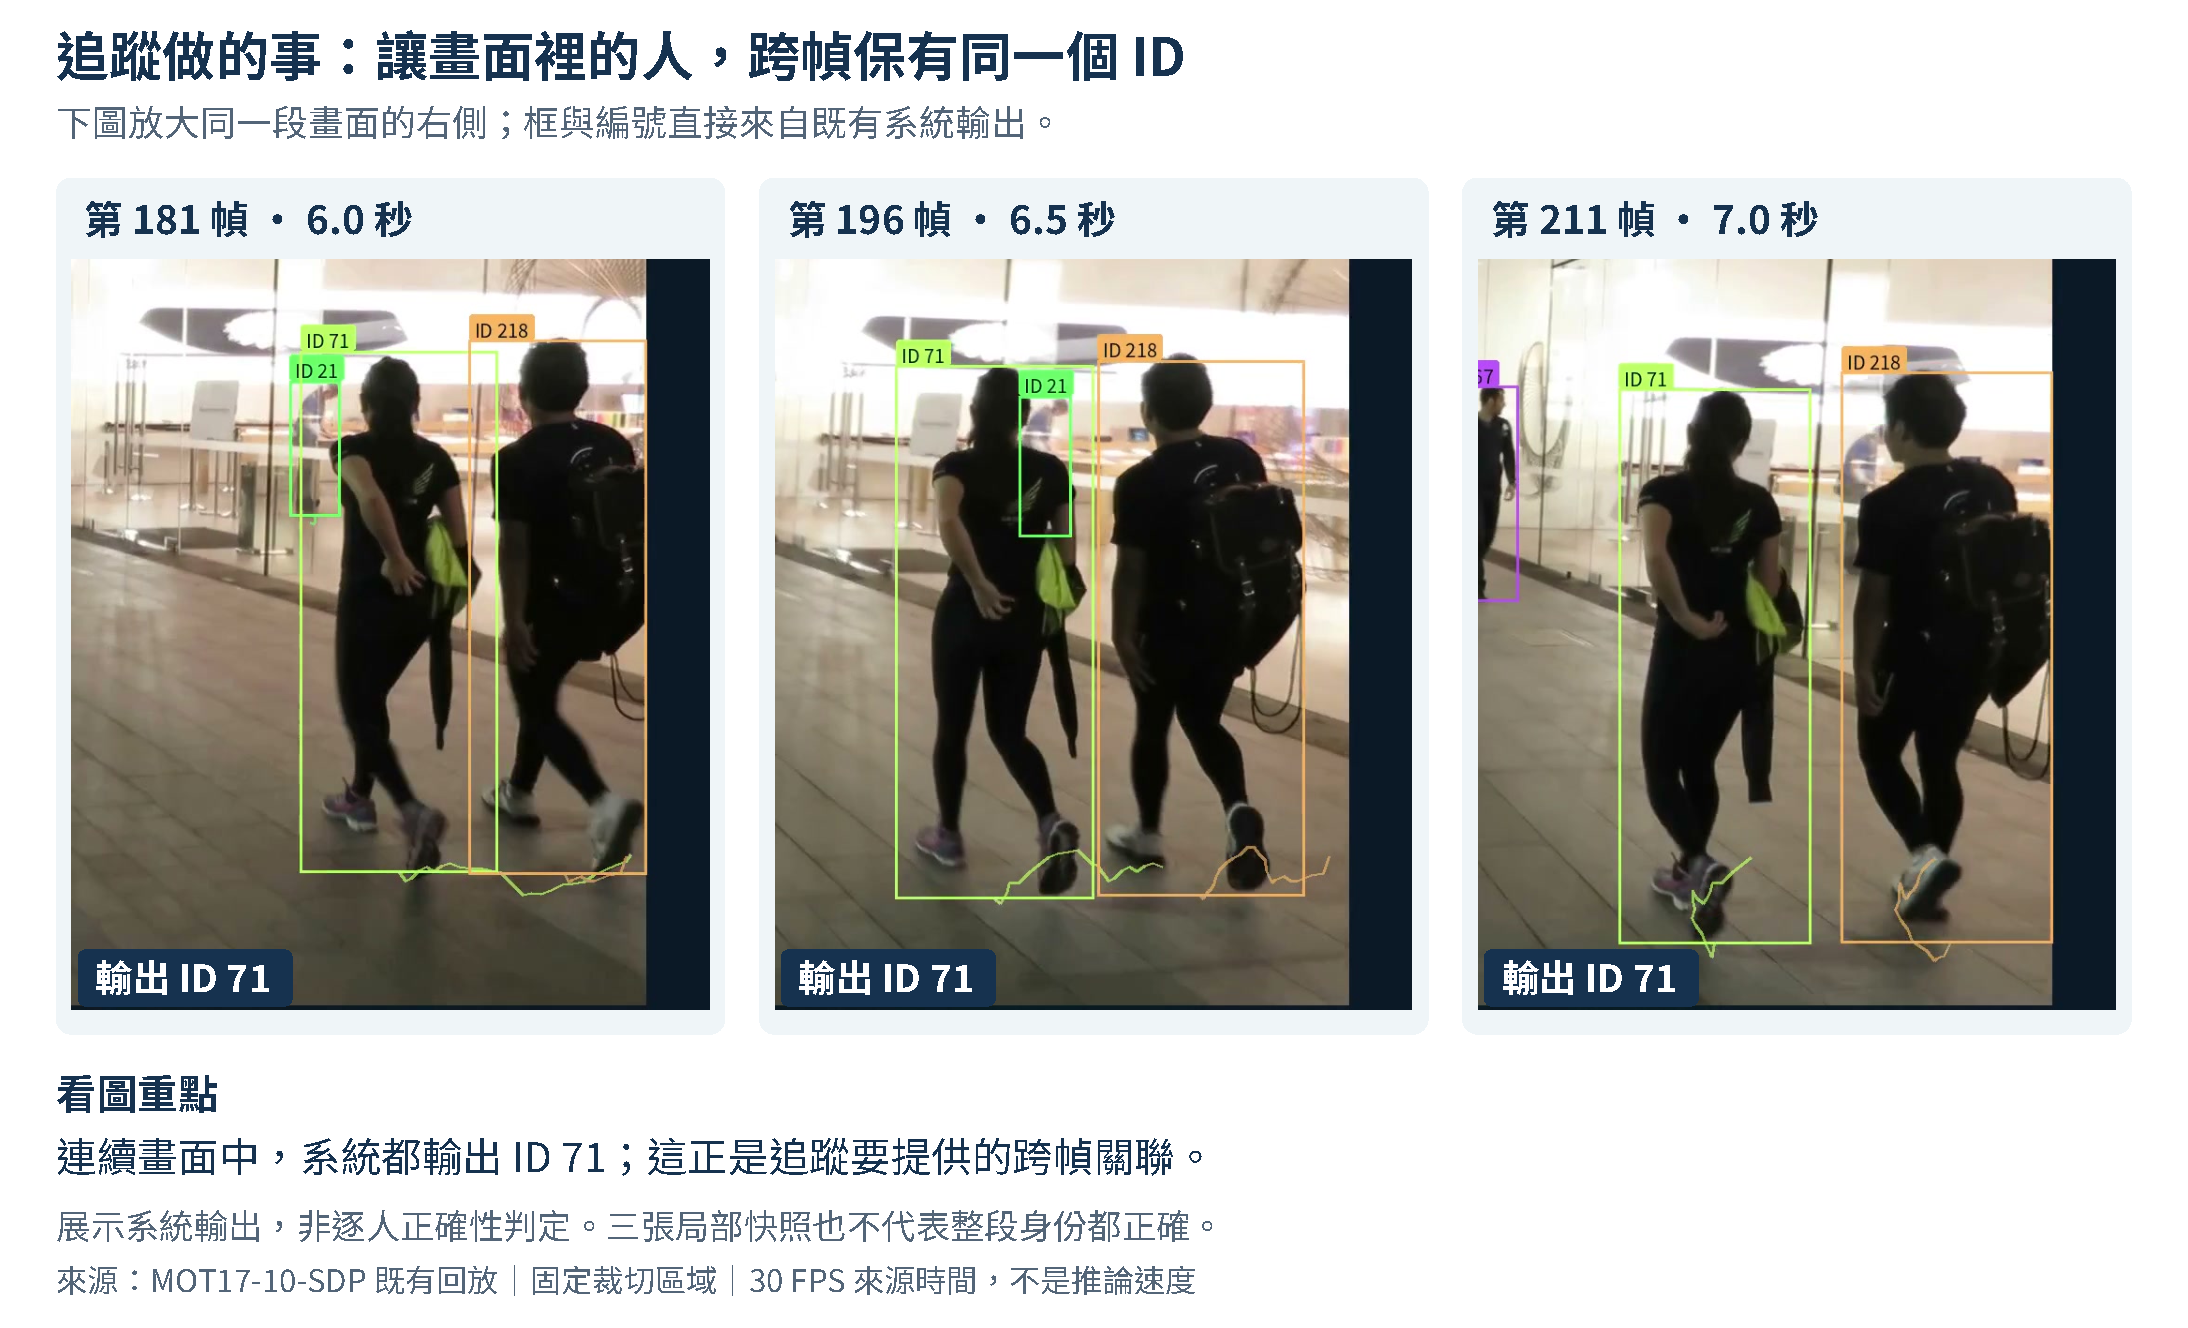
\includegraphics[width=\textwidth]{assets/story-example.pdf}
\caption{同一段影片的三個局部畫面。展示系統輸出，沒有以這三張圖判定整段追蹤是否正確。}
\end{figure}

\textbf{找人與接續身份是兩件工作。} 偵測器每幀找人；追蹤器用位置、運動和先前狀態把框接起來。漏掉幾幀、兩人靠近或遮擋，都可能讓 ID 中斷或接錯，所以「框得多」還不足以代表「身份接得穩」。

\textbf{相機也會動。} GMC 先估計背景整體的位移，把它放進目標位置預測，減少攝影機移動造成的干擾。它有明確的用途，效果仍要由資料判斷。

\textbf{Mamba 放在哪裡？} 現行模型在偵測 head 加入沿畫面空間掃描的分支；這是每幀的特徵處理。跨幀身份由追蹤器保存，沒有把 Mamba hidden state 當成影片身份記憶，也沒有額外的 ReID 外觀模型。\cite{tracking}

想自己看動態結果，可開啟專案中的展示台，逐幀查看框、ID 和相機位移：\path{docs/demos/report1/index.html}。圖中的 30 FPS 是展示影片播放速率，並非系統推論速度。

\clearpage
\section{n 和 n+1 為什麼能交錯？}
這裡的 n 是上一張畫面，n+1 是下一張。\textbf{下一幀的偵測路徑可以先往前走，上一幀繼續完成追蹤。} 目的在於利用兩條工作路徑的空檔，提高連續處理的效率。

\begin{figure}[H]
\centering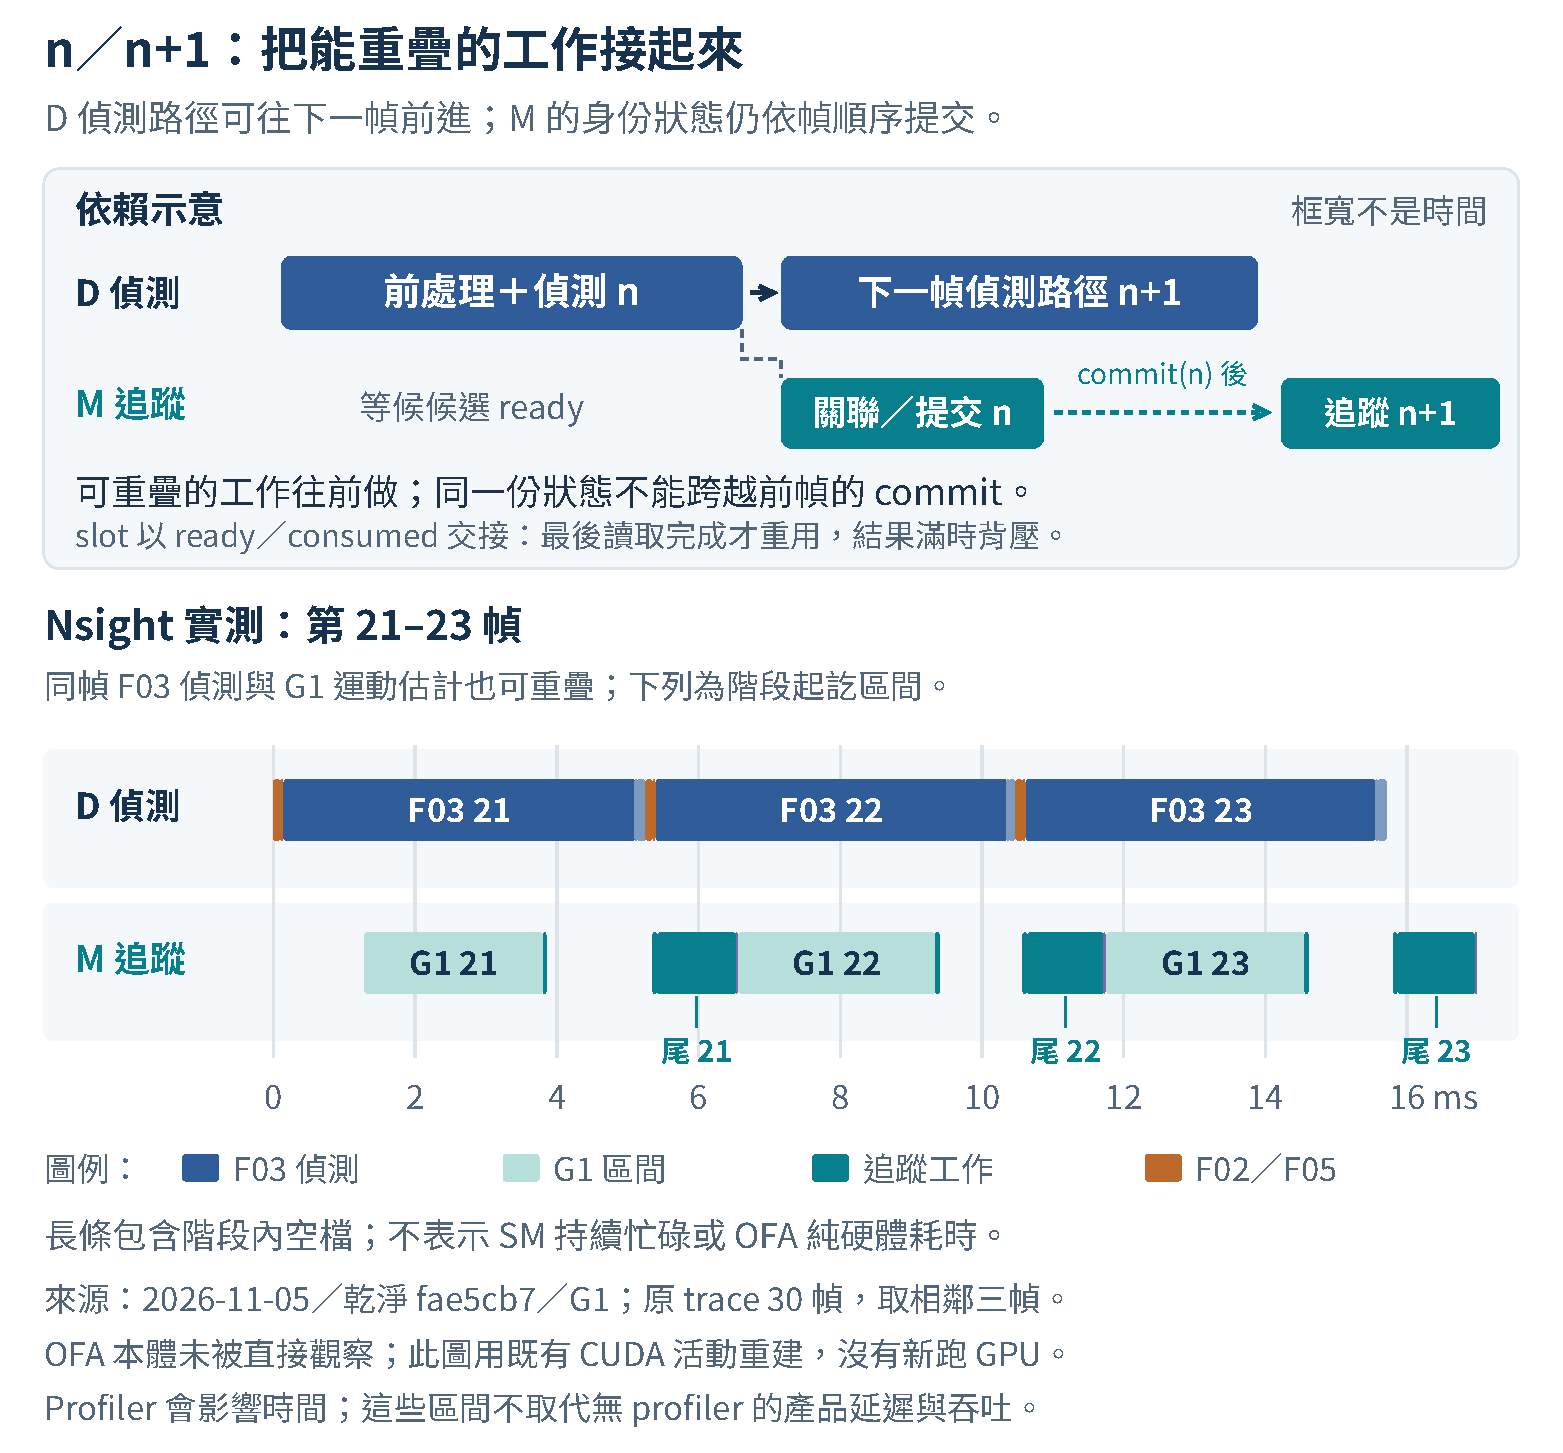
\includegraphics[width=\textwidth]{assets/story-schedule.pdf}
\caption{上半是依賴示意，下半由既有 G1 Nsight trace 重建；只有下半圖的橫軸代表實測時間。}
\end{figure}

% Recomputed from the archived G1 trace; see schedule-sources.json and schedule-trace/summary.json.
\textbf{實測看到了什麼？} 排除初始化與第一次 Execute 後，28 幀的完整 G1／F06 都落在同幀 F03 的時間窗內；27 組相鄰幀都有跨幀 CUDA 活動重疊，平均約 \textbf{0.94 ms}。主要交集是下一幀 F03 與上一幀的 mask／追蹤尾端。這是歷史 profiler trace 的排程觀察，產品延遲仍以無 profiler 的量測解讀。\cite{nsys}


\textbf{ID 狀態仍依序更新。} M(n+1) 要接在 M(n) 的 commit 之後，buffer 也要等讀取完成才可重用。兩條路徑可以交錯，不能把不同影格的狀態任意交換。\cite{tracking,nsys}

\clearpage
\section{哪些資料集有進步}
我們把官方預訓練 YOLO26m、微調 YOLO26m 和現行 HR Mamba 放進共用的前後處理與追蹤流程。\textbf{先比較同一資料集內三個模型的差別}，跨資料集的分數不當作場景難度排名。

\begin{figure}[H]
\centering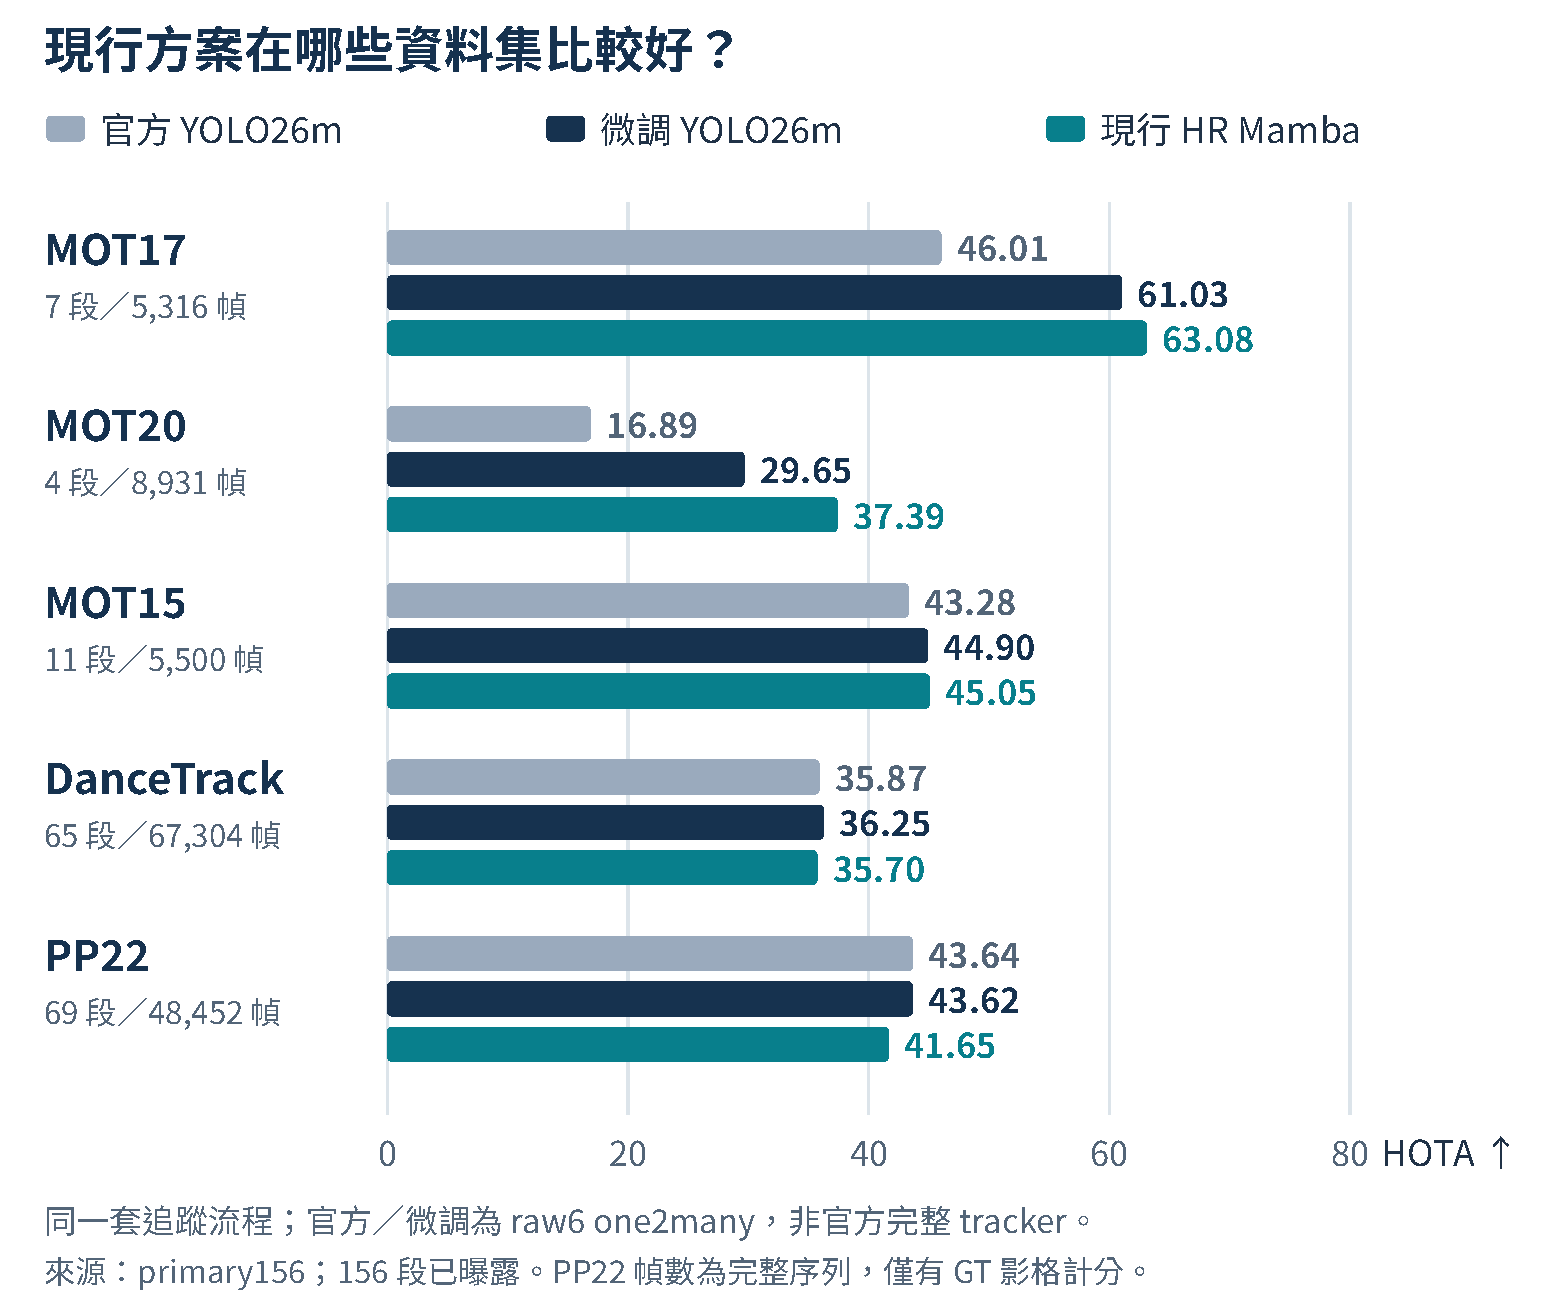
\includegraphics[width=\textwidth]{assets/story-datasets.pdf}
\caption{每模型 156 段、135,503 幀的既有結果。HOTA 同時看偵測與身份關聯，越高越好，但不是「追對百分之幾的人」。}
\end{figure}

相對微調 YOLO26m，HR 在 MOT17／MOT20 的合併 HOTA 增加約 \textbf{2.05／7.74 個百分點}；DanceTrack／PersonPath22 則下降約 \textbf{0.54／1.97}。MOT15 合併只小幅增加 0.15。

\textbf{MOT17 的合併分數含訓練序列。} 七段中的 04／05／09／11／13 是兩個本地模型的訓練序列，10 用來選模，只有 02 沒有參與訓練。02 的官方／微調／HR 為 36.76／37.71／40.57，HR 比微調高 2.86；選模用的 10 則是 HR 低 1.33（50.87 對 52.20）。官方到微調的 MOT17 合併差距約 15 個百分點，在 02 只剩 0.95，大部分來自訓練序列。

\textbf{這一輪看到的是場景差異。} MOT20 沒有參與兩個本地模型的訓練：微調版比官方高約 12.8，HR 再高 7.74，比 MOT17 合併值更能代表跨資料集表現。即使相對官方預訓練版，HR 在 DanceTrack 和 PersonPath22 也沒有比較高；不能把官方到現行模型的全部差距都算在 Mamba 上。\cite{primary156}

\clearpage
\section{為什麼還要拆開看}
合併數字方便閱讀，但容易遮住局部退步。例如 MOT15 整體略升，moving 子群卻下降。下圖把七個既定群組分開，以微調 YOLO26m 當零點。

\begin{figure}[H]
\centering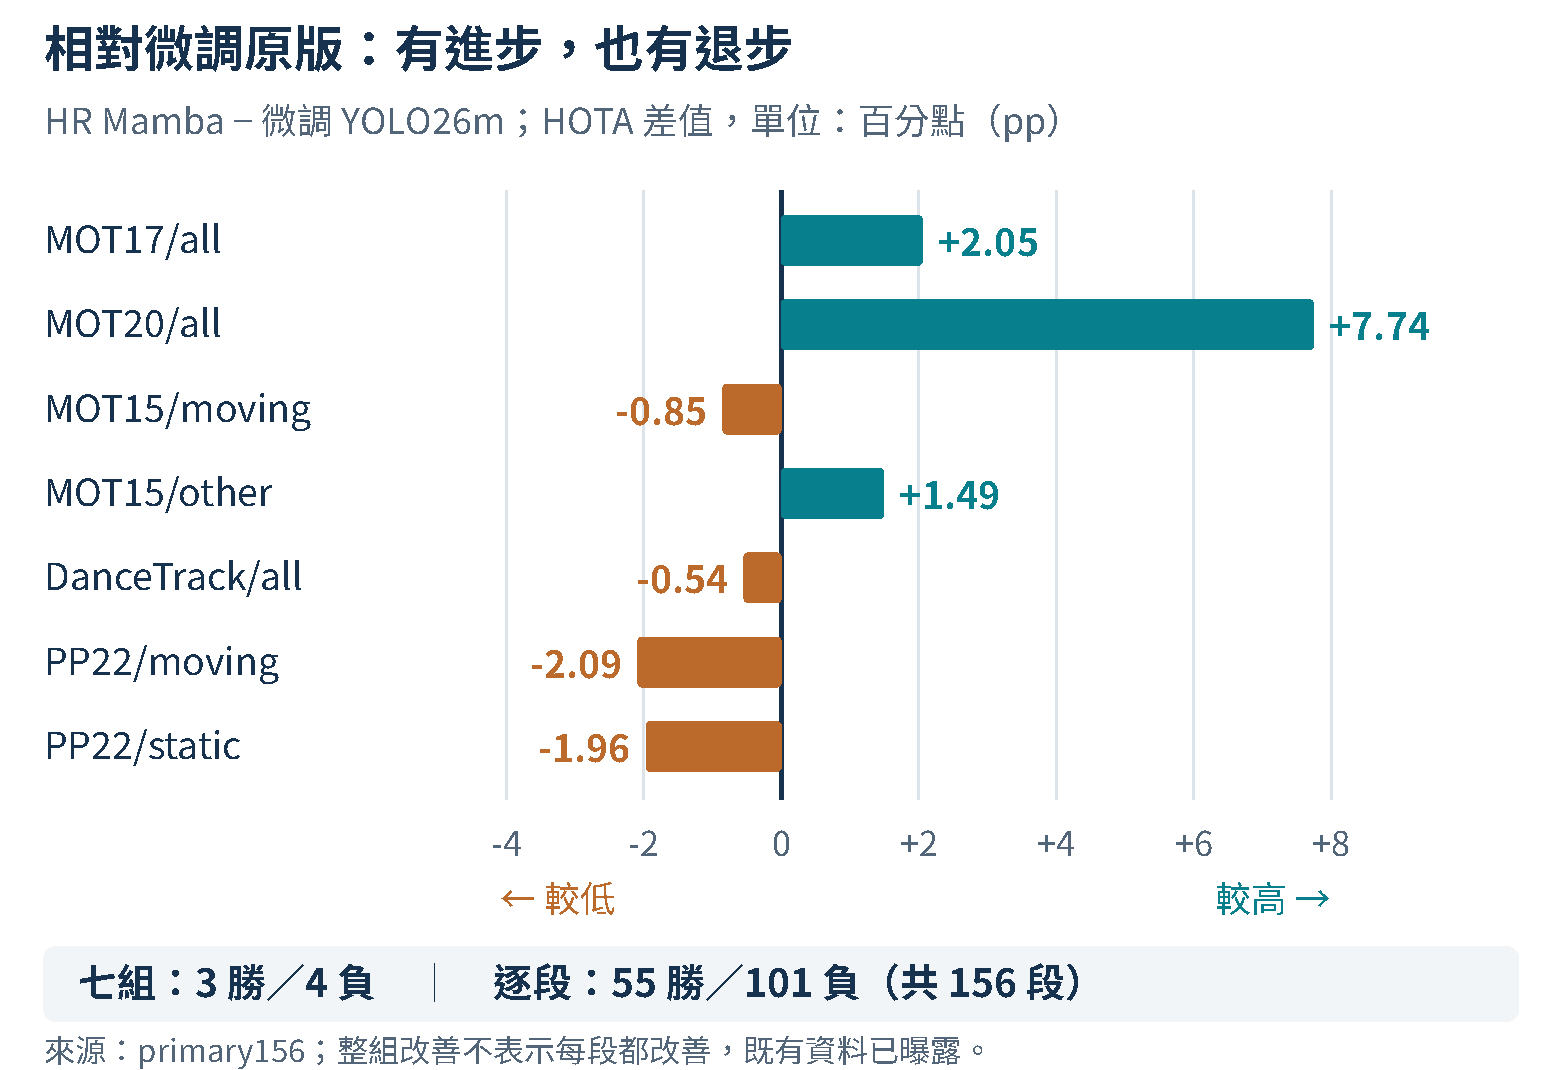
\includegraphics[width=\textwidth]{assets/story-group-deltas.pdf}
\caption{向右表示 HR 較高，向左表示 HR 較低。MOT17/all 含本地訓練與選模序列，見第 4 節。}
\end{figure}

\begin{finding}
\textbf{七組裡，3 組增加、4 組下降；逐段看是 55 段增加、101 段下降。}\par
MOT17／MOT20 的合併提升值得繼續理解，也要把其他群組的退步一起帶進判斷。
\end{finding}

\textbf{總分增加，也不表示身份切換變少。} MOT20 的四段 HOTA 都增加，合併 IDSW 卻從微調版 2,401 次增加到 HR 的 3,754 次；MOT17 也由 364 次增至 385 次。需要同時看偵測覆蓋、身份關聯和切換次數。

HOTA 看整體偵測與關聯，IDF1 看身份對應的一致性，IDSW 計算切換次數；這些角度會給出不同線索。完整數字保留在附表。\cite{primary156}

\clearpage
\section{這些品質差異，多花了多少時間}
速度另外量，只看兩個 MOT17 序列各自的前 140 幀；它回答固定條件下的計算取捨，不代表五個資料集的完整效能。

\begin{figure}[H]
\centering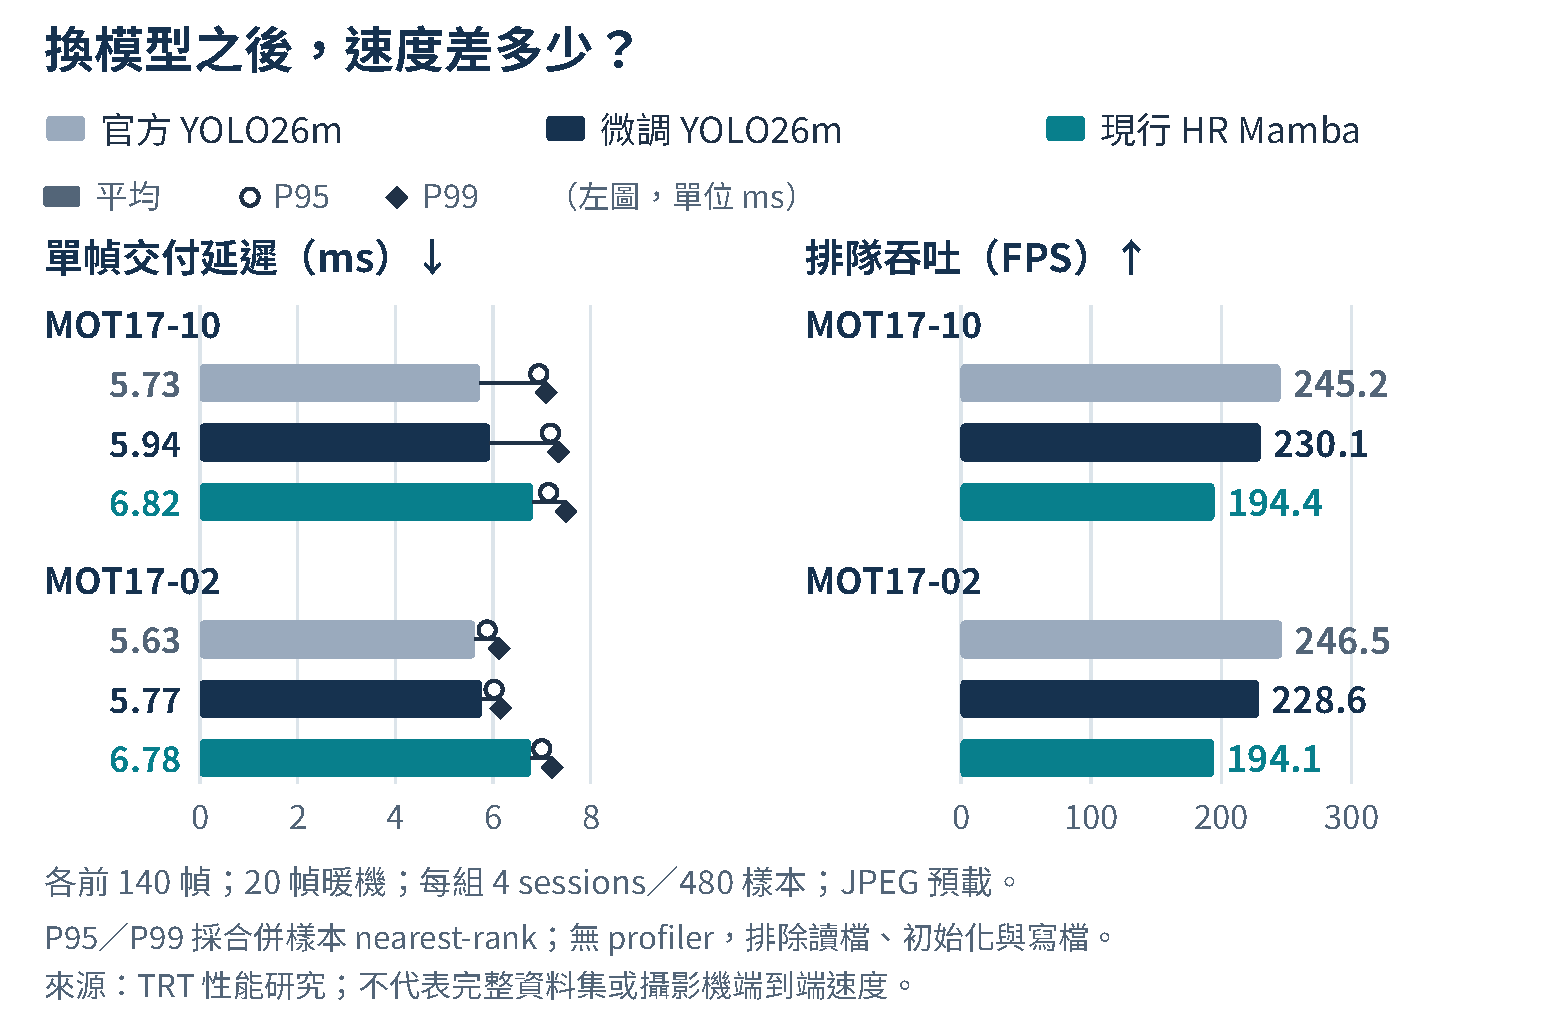
\includegraphics[width=\textwidth]{assets/story-speed.pdf}
\caption{左圖比較單幀平均值與 P95／P99，單位 ms；右圖為持續處理的 FPS。}
\end{figure}

\textbf{HR 每幀多約 0.9--1.0 ms，吞吐少約 15\%。} 相對微調 YOLO26m，HR 的 single 平均延遲在 MOT17-10／02 增加 14.79\%／17.42\%，queued 吞吐下降 15.52\%／15.13\%；F03 偵測本身增加 25.76\%，engine 檔案大 41.77\%（表 5）。\cite{trtcompare}

\textbf{P95／P99 看較慢的尾端}：這批樣本約 95\%／99\% 不超過該延遲，由四次 session 合併的 480 筆計算；queued 另含在途等待。Queued 尾端兩序列都是 HR 較高；single 尾端在 MOT17-10 與微調版相差不到 0.2 ms，時脈未鎖定、樣本有限，不足以判斷誰較穩。

% Generated from saved pipeline summary; modes remain separate.
\begin{table}[H]
\caption{逐幀交付延遲的 P95／P99（ms）；每組 480 筆合併樣本}
\small
\noindent\begin{tabularx}{\textwidth}{@{}P{21mm}Yrrrr@{}}
\toprule
序列 & 模型 & Single P95 & P99 & Queued P95 & P99 \\
\midrule
MOT17-10 & 官方 YOLO & 6.938 & 7.088 & 16.954 & 17.317 \\
MOT17-10 & 微調 YOLO & 7.178 & 7.339 & 19.908 & 20.529 \\
MOT17-10 & HR Mamba & 7.139 & 7.494 & 21.309 & 21.748 \\
MOT17-02 & 官方 YOLO & 5.882 & 6.126 & 16.761 & 16.994 \\
MOT17-02 & 微調 YOLO & 6.024 & 6.160 & 19.984 & 20.255 \\
MOT17-02 & HR Mamba & 6.999 & 7.214 & 21.216 & 21.539 \\
\bottomrule
\end{tabularx}
\end{table}


\clearpage
\section{這輪留下的答案}
\textbf{工程上，完整流程已接通。} C++／CUDA／TensorRT 主線可以從 JPEG 序列產生偵測、相機位移、追蹤 ID 與 MOT 結果。Runtime 不需要 Python；模型訓練與匯出工具另外使用 Python。展示台可以把這些輸出逐幀打開看。\cite{reference}

\textbf{模型上，還沒有一個全面勝出的答案。} 現行 HR 在未參與訓練的 MOT20 與 MOT17-02 較高，但平均延遲多約 15--17\%，DanceTrack／PersonPath22 也沒有跟著變好；MOT17 合併值含訓練序列，不能直接當成泛化。後續若要解釋 Mamba 的作用，需要把訓練配方、校準和架構因素分開；這份比較尚未做到只改架構一項因素。\cite{primary156,trtcompare}

\textbf{驗證上，有些問題仍然留著。} 輸出一致性和功能已有受測證據；完整記憶體／競態檢查還有未完成項目。真實相機或 RTSP 從輸入到消費端的完整延遲，也還沒有量完。這些限制會影響後續使用判斷，細項保留在技術版。\cite{reference}

\begin{finding}
\textbf{接下來值得釐清的問題}\par
哪些情況讓偵測改善卻多了身份切換？退步的群組有沒有共同特徵？如果實際場景更在意等待時間，應該怎麼選模型與排隊方式？
\end{finding}

這些是由本輪結果帶出的下一步問題，沒有在這次修訂啟動新實驗。現有模型和預設設定維持原樣。

\subsection*{想往下看，可以從這裡開始}
\begin{itemize}
\item \textbf{想看實際輸出：} 展示台 \path{docs/demos/report1/index.html}。
\item \textbf{想核對數字：} 後面的比較條件與完整附表，以及原始 JSON／CSV。
\item \textbf{想查怎麼實作：} 詳細稿 \path{docs/reports/report1-3cbaa518f0dc.md}，保留架構、同步與歷史測時。
\item \textbf{想查完整驗證：} 同目錄的 \path{technical-reference-v1.1.pdf}，保留原 20 頁技術報告及來源。
\end{itemize}

\appendix
\clearpage
\section{數字背後的比較條件}
這裡把需要一起引用的條件集中列出，主文圖表使用的是已完成的本機研究，本次只重畫圖、調整說明，沒有重跑推論、計分、訓練或調參。

\textbf{品質資料。} 五資料集共有 156 段，每模型 135,503 幀，三模型合計 468 cells。MOT17 為 train 目錄中七個不同 SDP 序列，MOT20 為 train 四段，MOT15 為 train 十一段，DanceTrack 為 train 40＋val 25 段，PersonPath22 為 mot\_test\_kf 69 段。Train 是資料集目錄名，本地兩條模型 lineage 的訓練分工另見原始 provenance。PP22 的 48,452 是完整序列幀數，計分只保留 8,753 個有 GT 的原始影格，原幀號不變。SportsMOT 排除主要推論、評分與選參。\cite{primary156}

\textbf{三方模型。} 官方為 YOLO26m 預訓練權重，微調版為 UA2 teacher e4 primary EMA，HR 為 Full25 mixed student e10 primary EMA。三方共用 native F01／F02、F04、G1 tracker，1280×768、batch 1、FP16 allowed、FP32 I/O；Graph ON，slots=2／2／4，NSA／量測框 OFF。各模型產生自己的偵測與 GMC。官方／微調採 raw6 one2many 接共用 tracker，並非官方預設 one2one 端到端流程。原始 one2one 只有另一次模型層控制，未混入這些品質圖。\cite{trtcompare}

\textbf{合併與資料曝光。} HOTA／DetA／AssA 使用完整 19-alpha raw arrays，IDF1／MOTA 使用各自正式 \code{combine_sequences}，不平均各段分數。這 156 段先前皆已曝光；MOT17 的 04／05／09／11／13 用於本地模型訓練，10 選模，02 是 M4 後重用的原 held-out。官方預訓練 corpus 未全面稽核。分數不代表獨立盲測或官方排行榜。\cite{primary156}

\textbf{測速條件。} RTX 5070 Ti Laptop、TensorRT 10.16.1.11；兩個 MOT17 prefix、每次 20 幀暖機＋120 幀量測、每模式四次 fresh sessions／480 samples。JPEG 預載，排除讀檔、初始化、暖機和寫檔，未鎖定 clocks。Single 量 enqueue 到 receive 返回，queued FPS 量整段完成吞吐；沒有用品質 capture wall time 推算資料集 FPS。\cite{trtcompare}

\textbf{尾延遲。} P95／P99 從四次 session 的逐幀 delivery 樣本合併後取 nearest-rank，480 筆分別取排序第 456／476 筆，不平均各 run 的分位數。原速度稽核核對 mean／P95；本次另從 48 份原始 CSV 獨立核對全部 12 組的 P95／P99，與保存摘要相同。收據見本目錄 \path{latency-percentiles-audit.json}；此輪未重新測速。

\textbf{排程圖。} 實測部分另用 2026-11-05、乾淨 \code{fae5cb7} 的 G1／HR 30 幀 Nsight trace 重算，並非上述三方測速，也不是在報告基準新增量測。Node capture 的 Graph 內 kernels 依 Graph 內容及 launch 對應回 D／M，不把 profiler 的 synthetic stream 當作實體 stream。Nsight 沒有直接觀察 OFA 本體，相關界限含排程與等待，不是純 OFA engine 延遲。\cite{nsys}

\textbf{數值與驗證限制。} 官方／微調 FP16 engine 的 1\% raw relative-L2 screen 仍為 FAIL，最大約 2.406\%／1.537\%。任務分數不能取代數值驗收。完整 G1 memcheck、原生完整 Graph racecheck、nvJPEG initcheck 等 OPEN／FAIL 保留；這次圖文修訂不關閉任何驗證項目。\cite{reference}

\clearpage
\section{完整品質與速度數字}
以下表格與主文圖表取自同一份保存分數；取三位小數，完整精度與 FP／FN／Frag 可查來源 JSON／CSV。IDSW 為次數，其餘品質欄位為百分點尺度；DetA 是 HOTA 的偵測指標，不能當成 AP50。\cite{primary156,trtcompare}
% Generated from the same saved metrics as model-comparison.tex.
\begin{table}[H]
\caption{資料覆蓋與 HOTA；Δ 為 HR 減比較對象（pp）}
\small
\noindent\begin{tabularx}{\textwidth}{@{}Yrrrrrrr@{}}
\toprule
資料集 & 段數 & 幀數 & 官方 & 微調 & HR & Δ 官方 & Δ 微調 \\
\midrule
MOT17 & 7 & 5,316 & 46.011 & 61.030 & 63.083 & +17.072 & +2.053 \\
MOT20 & 4 & 8,931 & 16.892 & 29.647 & 37.390 & +20.498 & +7.742 \\
MOT15 & 11 & 5,500 & 43.277 & 44.901 & 45.054 & +1.777 & +0.153 \\
DanceTrack & 65 & 67,304 & 35.869 & 36.245 & 35.702 & -0.167 & -0.543 \\
PP22 & 69 & 48,452 & 43.638 & 43.623 & 41.649 & -1.989 & -1.974 \\
\bottomrule
\end{tabularx}
\end{table}
\begin{table}[H]
\caption{完整品質數字；IDSW 是次數，其餘為百分點尺度}
\small
\noindent\begin{tabularx}{\textwidth}{@{}P{22mm}Yrrrrrr@{}}
\toprule
資料集 & 模型 & HOTA & DetA & AssA & IDF1 & MOTA & IDSW \\
\midrule
MOT17 & 官方 YOLO26m & 46.011 & 42.638 & 50.107 & 55.597 & 45.275 & 332 \\
MOT17 & 微調 YOLO26m & 61.030 & 63.036 & 59.670 & 71.329 & 73.291 & 364 \\
MOT17 & 現行 HR Mamba & 63.083 & 66.295 & 60.523 & 71.528 & 76.216 & 385 \\
MOT20 & 官方 YOLO26m & 16.892 & 8.196 & 34.995 & 15.976 & 9.598 & 418 \\
MOT20 & 微調 YOLO26m & 29.647 & 27.800 & 32.076 & 41.116 & 36.965 & 2401 \\
MOT20 & 現行 HR Mamba & 37.390 & 41.121 & 34.505 & 51.204 & 54.961 & 3754 \\
MOT15 & 官方 YOLO26m & 43.277 & 40.579 & 46.502 & 55.483 & 22.676 & 261 \\
MOT15 & 微調 YOLO26m & 44.901 & 41.253 & 49.103 & 56.522 & 19.777 & 211 \\
MOT15 & 現行 HR Mamba & 45.054 & 41.218 & 49.557 & 56.816 & 19.178 & 211 \\
DanceTrack & 官方 YOLO26m & 35.869 & 60.478 & 21.515 & 36.675 & 74.088 & 7734 \\
DanceTrack & 微調 YOLO26m & 36.245 & 61.008 & 21.775 & 37.520 & 76.594 & 7646 \\
DanceTrack & 現行 HR Mamba & 35.702 & 59.367 & 21.702 & 37.431 & 73.996 & 8318 \\
PP22 & 官方 YOLO26m & 43.638 & 45.211 & 42.521 & 48.216 & 47.942 & 4517 \\
PP22 & 微調 YOLO26m & 43.623 & 45.663 & 42.240 & 50.269 & 43.333 & 4484 \\
PP22 & 現行 HR Mamba & 41.649 & 44.103 & 39.914 & 47.947 & 39.138 & 5138 \\
\bottomrule
\end{tabularx}
\end{table}
\begin{table}[H]
\caption{七個既定群組；逐段勝／平／負為 HR 相對微調版}
\small
\noindent\begin{tabularx}{\textwidth}{@{}Yrrrrrr@{}}
\toprule
群組 & 段數 & 官方 & 微調 & HR & Δ 微調 & 勝／平／負 \\
\midrule
MOT17/all & 7 & 46.011 & 61.030 & 63.083 & +2.053 & 4/0/3 \\
MOT20/all & 4 & 16.892 & 29.647 & 37.390 & +7.742 & 4/0/0 \\
MOT15/moving & 5 & 40.244 & 44.184 & 43.335 & -0.849 & 1/0/4 \\
MOT15/other & 6 & 47.116 & 45.783 & 47.275 & +1.492 & 1/0/5 \\
DanceTrack/all & 65 & 35.869 & 36.245 & 35.702 & -0.543 & 29/0/36 \\
PP22/moving & 9 & 45.152 & 44.694 & 42.607 & -2.087 & 2/0/7 \\
PP22/static & 60 & 43.527 & 43.546 & 41.581 & -1.965 & 14/0/46 \\
\bottomrule
\end{tabularx}
\end{table}
\begin{table}[H]
\caption{MOT17-10 前 140 幀；F03 和完整 tracking 分開測量}
\small
\noindent\begin{tabularx}{\textwidth}{@{}Yrrrrr@{}}
\toprule
模型 & F03 ms & Single mean ms & Single p95 ms & Queued FPS & Engine MiB \\
\midrule
官方 YOLO26m & 3.744 & 5.734 & 6.938 & 245.175 & 42.506 \\
微調 YOLO26m & 3.809 & 5.938 & 7.178 & 230.123 & 40.868 \\
現行 HR Mamba & 4.790 & 6.816 & 7.139 & 194.417 & 57.939 \\
\bottomrule
\end{tabularx}
\end{table}


\clearpage
\begin{thebibliography}{9}
\footnotesize
\setlength{\itemsep}{0.3em}
\bibitem{tracking} 流程與模型實作：\path{docs/TRACKING.md} §20、\path{src/tracking_session.cpp}、\path{src/head_trt_network.cpp}。架構圖與實作對照見詳細稿。
\bibitem{primary156} 五資料集／七群組品質研究，2026-11-11。\newline\path{evidence/model-comparison/2026-11-11-yolo26m-primary156/bundle/REPORT.md}；同包 \path{metrics/summary.json}、\path{metrics/per-sequence.csv}、\path{audits/scoring-audit.json}、\path{training-provenance.json}、\path{evaluation-scope.json}。
\bibitem{trtcompare} 三模型 TensorRT 速度與品質比較，2026-11-11。\newline\path{evidence/model-comparison/2026-11-11-yolo26m-trt-performance/REPORT.md}；同包 \path{performance/pipeline/summary.json}、\path{performance/model/summary.json}、\path{comparison.json}、\path{validation.json}。
\bibitem{reference} 原 v1.1 完整技術報告與原稿保留於本目錄 \path{technical-reference-v1.1.pdf}、\path{technical-reference-v1.1.tex}；來源映射與 hashes 見 \path{technical-reference-v1.1.json}。對應原始階段證據、量測收據與 OPEN 範圍均保留。
\bibitem{nsys} G1 排程 trace 重算與連續影格時間軸，2026-11-12。\newline\path{evidence/report1/2026-11-12-schedule-trace/}；來源為 \path{evidence/tracking-session/2026-11-05-v1-motion-2-acceptance-2/capture/nsys.sha256} 指定的原始 node／graph trace，受測 \code{fae5cb7}。本次未新增 GPU capture。
\end{thebibliography}
\end{document}
